%
%                       This is a LaTeX 2e version of the
%                       laboratory project template file.
\documentclass[a4paper,12pt]{article}
\usepackage{fullpage, graphicx}
\usepackage[backend=biber, style=nature, sorting=none]{biblatex}
\addbibresource{references/ESTproject.bib}
\usepackage{subcaption}
\usepackage{amsmath}
\usepackage{listings}
\usepackage{color} %red, green, blue, yellow, cyan, magenta, black, white
\usepackage{siunitx}
\definecolor{mygreen}{rgb}{0,0.6,0}
\definecolor{mygray}{rgb}{0.5,0.5,0.5}
\definecolor{mymauve}{rgb}{0.58,0,0.82}

\lstset{ %
	backgroundcolor=\color{white},   % choose the background color
	basicstyle=\footnotesize,        % size of fonts used for the code
	breaklines=true,                 % automatic line breaking only at whitespace
	captionpos=b,                    % sets the caption-position to bottom
	commentstyle=\color{mygreen},    % comment style
	escapeinside={\%*}{*)},          % if you want to add LaTeX within your code
	keywordstyle=\color{blue},       % keyword style
	stringstyle=\color{mymauve},     % string literal style
}

\graphicspath{{images/}}

\DeclareUnicodeCharacter{2212}{-}
%
%                       This section generates a title page
%                       Edit only the sections indicated to put
%                       in the project title, your name, supervisor,
%                       project length in weeks and submission date
%
\begin{document}
\pagestyle{empty}                       % No numbers of title page
\begin{minipage}[b]{110mm}
        {\Huge\bf School of Physics\\ and Astronomy
        \vspace*{17mm}}
\end{minipage}
\hfill
\begin{minipage}[t]{40mm}               
        \makebox[40mm]{
        
\includegraphics[width=4cm]{crest.pdf}}
\end{minipage}
\par\noindent                                           % Centre Title, and name
\vspace*{1cm}
\begin{center}
        \Large\bf \Large\bf Electronic Structure Theory\\
        \Large\bf Project 1\\[10pt]                     % Change to MP/CP/Astro
        \vspace*{0.3cm}
        \LARGE\bf High Temperature Superconductivity\\        % Change to suit
        \large \bf of\\
        \large \bf High Pressure H$_3$S
\end{center}
\vspace*{0.3cm}
\begin{center}
        \bf Declan Mathews\\                           % Repace with your name
        \today                             % Submission Date
\end{center}
\vspace*{3mm}
%
%                       Insert your abstract HERE
%                       
\begin{abstract}
	%      The abstract is a short, concise explanation of the project
    %    covering the aims, outlines of techniques used and a short
    %    summary of the results. It should contain enough information to
    %    make the aims and success of the project clear, but contain no details.
    %    A typical abstract should be between 50 and 100 words.
       \noindent This report looks to estimate the superconducting temperature $T_c$ of the \textit{Im-3m} high pressure phase of H$_3$S at 200 GPa. This estimate will found via BCS theory using the McMillan-Allen-Dynes equation and look to reproduce the results from Duan 2014 with a $T_c$ of 191 K to 204 K for a Coulomb screening potential value $\mu^*=0.10-0.13$. The results here find a $T_c$ estimate of 180 K to 210 K for $\mu^*=0.10$ which is in good agreement with the original paper. This study was carried out using the QuantumESPRESSO package.
        
\end{abstract}

\vspace*{0.5cm}

\subsubsection*{Declaration}

\begin{quotation}
\noindent I declare that this project and report is my own work.
\end{quotation}

\vspace*{1.5cm}
Signature: Declan Mathews\hspace*{7cm}Date: 09/04/2020

                                       % Change to suit
\newpage
%
%                       End of Title Page
\tableofcontents                                % Makes Table of Contents
%\newpage
\pagestyle{plain}                               % Page numbers at bottom
\setcounter{page}{1}                            % Set page number to 1

\section{Introduction}
% aims
In recent history there have been many propositions and studies of different structures in an attempt to find a high critical temperature ($T_c$) superconductor. More specifically, the goal is to find a room temperature superconductor which can be used in place of standard conductors to substantially improve the efficency of energy transport. This is achieved as superconductors provide zero resistance and so produce substantially less waste heat energy. The first high temperature superconductors were found by Bednorz and M\"{u}ller (1986), with a copper oxide compound achieving a $T_c=35.1$ K \cite{bednorz_muller}. This prompted focus of the research towards various ceramic metal cuprates (metals exhibiting a layered structure) and there has been much success in achieving higher critical temperatures.

\bigskip

\noindent In 2015, Dihydrogen sulphide (H$_2$S) was found to be superconducting up to 203 K under a pressure of 150 GPa \cite{Drozdov_2015}. This follows a prediction from 2014 that at high pressures H$_2$S would decompose into sulphur and H$_3$S, with a high $T_c$ superconducting phase \textit{Im-3m}, as shown in Figure \ref{fig:im3m}. This structure is notably not layered but instead highly symmetrical and thought to exhibit superconductivity due to electron-phonon coupling, described well by Bardeen-Cooper-Schrieffer (BCS) theory \cite{BCS}. The prediction was a $T_c$ of 191 K to 204 K at 200 GPa \cite{duan} and having taken the step past 200 K this has prompted much research into hydride compounds.

 \begin{figure}[h!!!]
 	\centering
 	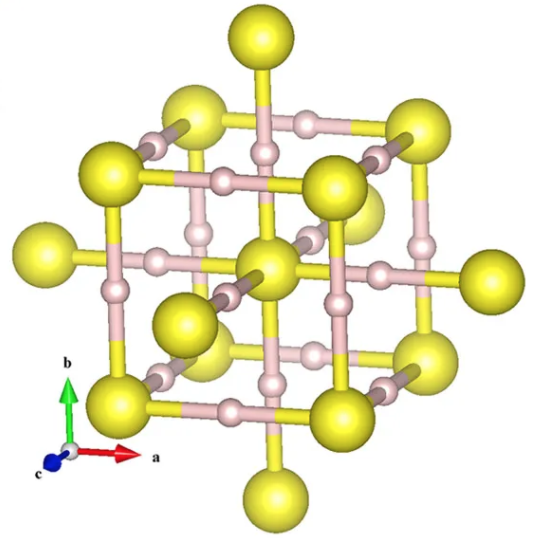
\includegraphics[width=10cm]{H3s_im-3m}
 	\caption{The \textit{Im-3m} phase of H$_3$S. The yellow spheres are sulphur atoms and the white spheres are hydrogen atoms. This image is taken from \cite{duan}}
 	\label{fig:im3m}
 \end{figure}

\bigskip

\noindent This report will focus on this \textit{Im-3m} phase of H$_3$S (lattice parameter $a = 2.984 \AA$ at 200 GPa) and look to estimate its superconducting temperature under BCS theory in an attempt to achieve similar results predicted in the 2014 paper. This should provide further validity and support the focus of research on hydrides and electron-phonon coupling as a primary focus for the mechanism of room temperature superconductivity (RTSC). The \textit{Im-3m} structure used is the same as theorised in Duan's 2014 paper. Various convergence tests have been ran using the Density Functional Theory (DFT) framework and the phonon dispersion calculated with Density Functional Perturbation Theory (DFPT). The Eliashberg function was used to determine the real force constants before finally using the McMillan-Allen-Dynes equation to determine an estimate for $T_c$.
 

\section{Methodology}
% Brief overview of DFT and concept of DFPT

\subsection{Density Functional Theory}
% Hoenberg-Kohn thms, Kohn-Sham eqns, self-consistent field cycle, LDA GGA PBE, Basis sets - Bloch thm, Pseudo-potentials - PAW, Brillouin zone sampling
DFT is an effective computational method to solve the many electron problem, whose hamiltonian can be written:

\begin{equation}
H_{el} = T_e + V_{ee}(\vec{r}) + V_{en}(\vec{R}, \vec{r}) + V_{nn}(\vec{R})
\end{equation}

\smallskip
\noindent Where $T_e$ is the kinetic energy of the electrons, $V_{ee}(\vec{r})$ is the electron-electron interaction potential, $V_{en}(\vec{R}, \vec{r})$ is the electron-nuclei interaction potential and $V_{nn}(\vec{R})$ is the nuclei-nuclei interaction potential.

\bigskip
\noindent This equation can be viable for single small atoms or molecules but when attempting to determine bulk properties of larger systems this involves too many terms to be feasible. DFT provides a framework to approximate the system and is based on two theorems laid out by Hoenberg and Kohn \cite{hk_thm}. These are as follows:

\begin{enumerate}
	\item For a system of interacting particles, the ground state density uniquely determines the external potential up to a constant value.

	\item The energy functional for an external potential is minimised by the exact ground state density, with a global minimum at the exact ground state energy.
\end{enumerate}

\noindent These theorems infer two key points; ground state observables are functionals of the ground state density and there is a unique functional for the ground state energy as follows:

\begin{equation}
E_o[n] = F_{HK}[n] + \int V_{en}(\vec{r})n(\vec{r})d\vec{r} + V_{nn} \\
\end{equation}
\[
F_{HK}[n] = \langle\psi_0[n]|T_e + V_{ee}|\psi_0[n]\rangle
\]

\smallskip
\noindent Where $\psi_0[n]$ is the ground state wavefunction defined as a functional of the electron density and $n(\vec{r})$ is the electron density as a function of position.

\bigskip
\noindent A final ansatz laid out by Kohn and Sham states that the system can be treated as non-interaction quasi-electrons with the same ground state density in an effective potential. This allows the above equations to be written in a form where variation of energy can be carried out, leading to the effective potential for single particles $V_{KS}$, giving the Kohn-Sham equations \cite{ks_eqns}:

\begin{equation}
\left[ -\frac{1}{2}\nabla^2 + V_H(\vec{r}) + V_{xc}(\vec{r}) + V_{en}(\vec{r}) \right] \phi_i(\vec{r}) = \epsilon_i \phi_i(\vec{r})
\end{equation}
\[
V_H\equiv\frac{\delta E_H}{\delta n}, \; V_{xc}\equiv\frac{\delta E_{xc}}{\delta n}, \; n(\vec{r})=\sum_{i=1}^{N}|\psi_i(\vec{r})|^2
\]

\smallskip
\noindent Where $V_H$ is the Hartree potential and $V_{xc}$ is the exchange correlation potential, which contains all unknown quantities. The bracketed terms is the Kohn-Sham potential $V_{KS}$. The total wave function is a product state of the single particle solutions.

\bigskip
\noindent These equations describe a self-consistent field (SCF) solution in which an iterative process can be implemented to find the ground state density which defines the ground state energy. The process is as follows:

\begin{enumerate}
	\item Define an initial trial electron density $n(\vec{r})$
	\item Solve the Kohn-Sham equations for the single particle wavefunctions $\psi_i(\vec{r})$
	\item Calculate the Kohn-Sham electron density $n_{KS}(\vec{r})$ from $\psi_i(\vec{r})$
	\item If $n_{KS}(\vec{r}) = n(\vec{r})$, this is the ground state electron density $n_0(\vec{r})$. If they are different repeat from step 1.
\end{enumerate}

\noindent Several methods of updating the trial electron density in each iteration have been developed. Among the most common are Local Density Approximations (LDA), which make use of the local electron density to estimate the a new trial density, and Generalised Gradient Approximations (GGA), which use the local density and local gradient of the density. A particularly common GGA method is the Perdew-Burke-Ernzerhof (PBE) method \cite{pbe} which was used in this study.

\bigskip
\noindent To represent the wavefunctions it is common to take advantage of Bloch's Theorem for periodic systems and use a plane-wave basis (as done here):

\begin{equation}
\psi_k(\vec{r}) = u(\vec{r}) \exp(i\vec{k}\cdot\vec{r})
\end{equation}
\[
u(\vec{r}) = \sum_{G}c(\vec{G})\exp(i\vec{G}\cdot\vec{r})
\]

\noindent This allows a cut-off energy to be introduced which can be tailored to suit a required convergence while reducing the data set size of the calculation. The cut off energy is determined by:

\begin{equation}
E_{cut}=\frac{1}{2}|\vec{k}+\vec{G}_{max}|^2
\end{equation}

\bigskip
\noindent Another optimisation to the wavefunction representation is the use of pseudo-potentials Core electrons and valence electrons in the core are not relevant to bonding in solids and so calculating them is unnecessary. Instead the Coulomb potential can be replaced with a pseudo-potential that leads to simpler basis set expansions. One method of doing so is the Projector Augmented Wave (PAW) method which is used in this study.

\bigskip
\noindent Finally, in order to gain an accurate result without too much computational expense, Brillouin zone sampling is used on a regular isotropic mesh ($N_k$, $N_k$, $N_k$) which can be tuned to produce results with a determined convergence This involves sampling various points through reciprocal space, which are assumed to represent the total space in the calculation.

\subsection{Density Functional Perturbation Theory}
% Linear response of KS, Hellman-Feynman thm, sternheimer eqns, Electron-phonon coupling, McMillen-Allen-Dynes, BCS 
The key idea in DFPT is to study the linear response of the Kohn-Sham system to a perturbation. To solve this, a set of self-consistent equations for the perturbed system is used known as the Sternheimer equations \cite{sternheimer}:

\begin{align}
\begin{split}
\left[ H_{el} - \epsilon_i \right] |\Delta\phi_i\rangle &= -\left( \Delta V_{KS} - \Delta\epsilon_i \right)|\Delta\phi_i\rangle \\
\Delta V_{KS}(\vec{r}) &= \Delta V_{en}(\vec{r}) + \int\frac{\Delta n(\vec{r}^{\prime})}{|\vec{r}-\vec{r}^{\prime}|}d\vec{r}^{\prime} + \int\frac{dV_{xc}(\vec{r}^{\prime})}{dn(\vec{r}^{\prime})}\Delta n(\vec{r}^{\prime})d\vec{r}^{\prime} \\
\Delta\epsilon_i &= \langle\phi_i|\Delta V_{KS}|\phi_i\rangle \\
\Delta n(\vec{r}) &= 2\sum_{i}f_i\phi_i^*(\vec{r})\Delta\phi_i(\vec{r})
\end{split}
\end{align}

\noindent Where the wavefunction perturbation is $\Delta\psi_i$, the potential perturbation is $\Delta V_{KS}$, the energy eigenvalue perturbation is $\Delta\epsilon_i$ and the electron density perturbation is $\Delta n(\vec{r})$.

\bigskip
\noindent The periodic phonon perturbations with wave vector \textbf{\textit{q}} couple electrons at all pairs (\textbf{\textit{k}}, \textbf{\textit{k}}+\textbf{\textit{q}}) and can be found by the following steps:

\begin{enumerate}
	\item Standard ground state calculation on regular \textbf{\textit{k}}-point grid for unperturbed wave functions and density.
	\item Solve Sternheimer equations for regular \textbf{\textit{q}}-point grid such that \textbf{\textit{k}}+\textbf{\textit{q}} are also in \textbf{\textit{k}}-grid.
	\item Determine $\Delta n(\textbf{\textit{q}})$, from which the force constant matrix can be found.
	\item Fourier transform the force constant matrix for the real-space interatomic force constants.
\end{enumerate}

\noindent As an extension to this, one can calculate an estimate for $T_c$ in BCS theory by following three further steps:

\begin{enumerate}
	\item By double summing over the \textit{\textbf{k}}-grid, calculate the electron-phonon coupling matrix element $g$ for each coupled pair and phonon branch $j$
	\item Integrate over the \textit{\textbf{q}}-grid and phonon branches to determine the Eliashberg function $\alpha^2F(\omega)$, electron-phonon coupling strength $\lambda$ and the weighted logarithmic average of the phonon frequency $\omega_{log}$.
	\item Finally, using the determined values and a value for the screened Coulomb potential $\mu^*$, an estimate for $T_c$ can be obtained using the McMillan-Allen-Dynes equation.
\end{enumerate}

\noindent The McMillan-Allen-Dynes equation is:

\begin{align}
\begin{split}
T_c &= \frac{\omega_{log}}{1.2}\exp\left[ -\frac{1.04(1+\lambda)}{\lambda + \mu^*(1+0.62\lambda)}\right] \\
\lambda &= 2\int\frac{\alpha^2F(\omega)}{\omega}d\omega \\
\omega_{log} &= \exp\left[ \frac{2}{\lambda}\int_0^{\infty}\frac{d\omega}{\omega}\alpha^2F(\omega)\ln\omega\right]
\end{split}
\end{align}

\noindent Where the integral for $\lambda$ is over the Fermi surface. The Eliashberg function $\alpha^2F(\omega)$ is not included here as it is not the focus of the study but can be found at \cite{estslides}. It is worth noting that is represents the frequency dependent electron coupling strength.

\section{Results}


\subsection{SCF Convergence Tests}
The results for the energy convergence per atom of the system are shown in Figure \ref{fig:E-conv}. These were found through carrying out the SCF step for $E_{cut} = 25 ... 100$ Ry in steps of 5 Ry. The energy of the 100 Ry solution was assumed to be fully converged and all other results shown are the difference from this value. $E_{cut} = 30$ Ry was chosen for use in this study as it fell within the desired 10 meV per atom convergence. The 1 meV per atom convergence is also noted for reference.

\begin{figure}[h!!!]
	\begin{subfigure}{0.5\textwidth}
	\centering
	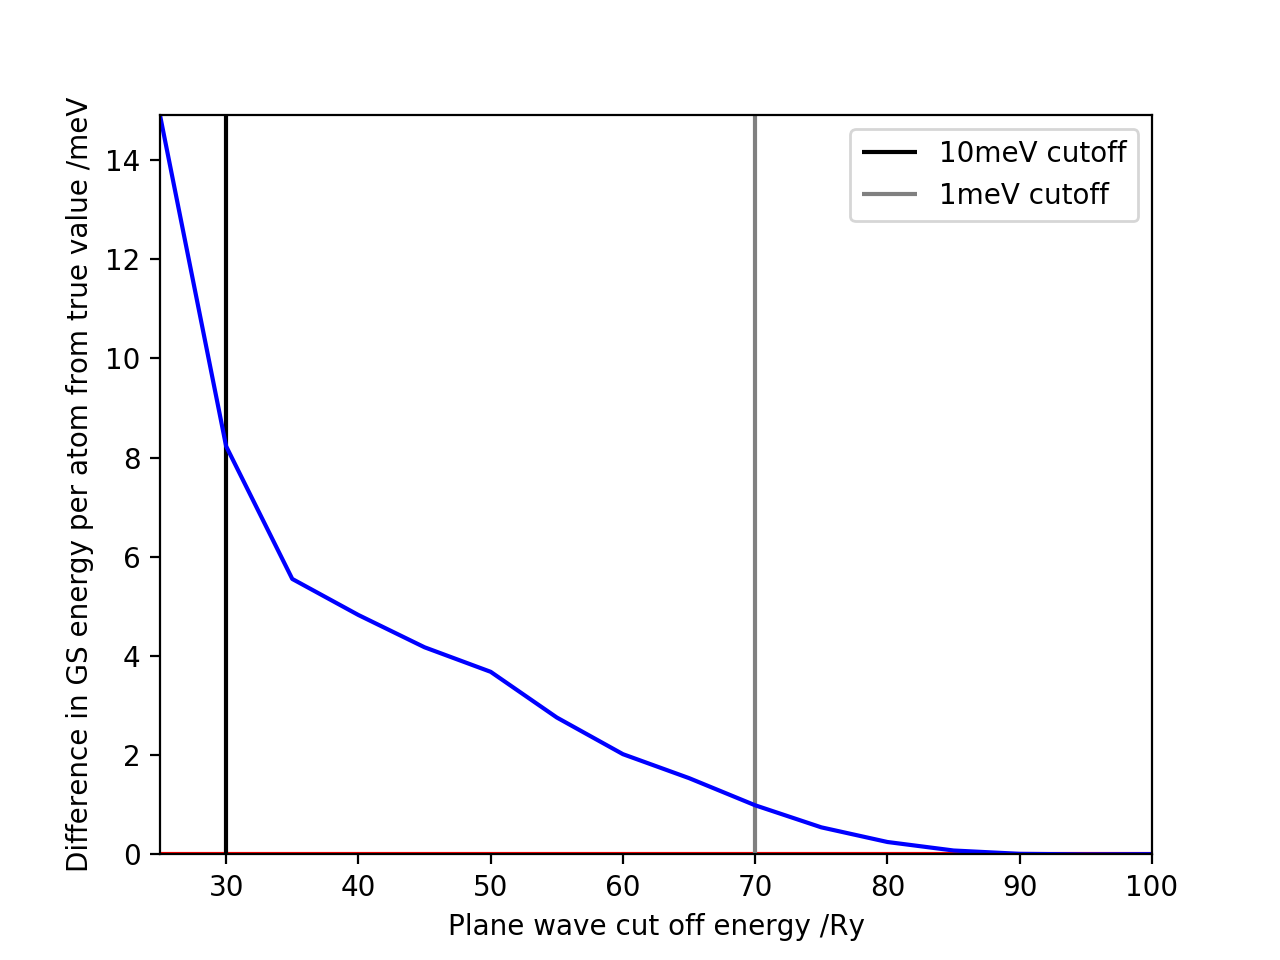
\includegraphics[width=8cm]{E-conv.png}
	\subcaption{ }
	\label{fig:E-conv}
	\end{subfigure}%
	\begin{subfigure}{0.5\textwidth}
	\centering
	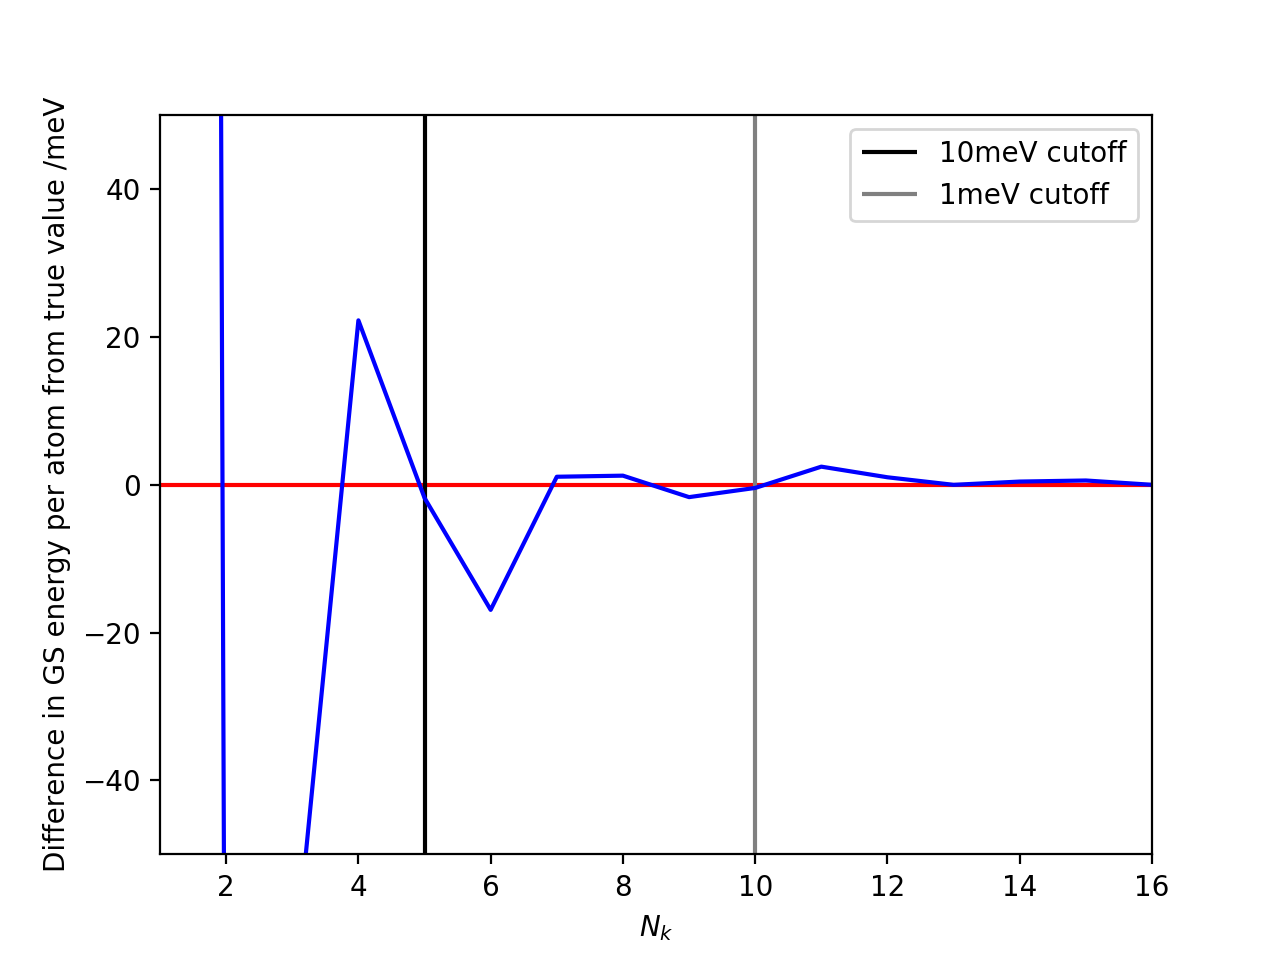
\includegraphics[width=8cm]{k-conv-zoom.png}
	\subcaption{ }
	\label{fig:k-conv}
\end{subfigure}%
\caption{The energy convergence per atom when varying (a) $E_{cut}$ values (b) the isotropic \textbf{\textit{k}}-point mesh. Note that $N_k$ is the number of points per axis ($N_k$, $N_k$, $N_k$). The final result is taken and the converged solution to compare all results to.}
\label{fig:scf}
\end{figure}

\bigskip
\noindent Figure \ref{fig:k-conv} shows the results for the energy convergence per atom when varying the isotropic \textbf{\textit{k}}-point mesh. The grid density was varied by changing the number of points sampled per axis $N_k$.

\subsection{Density of States Convergence Check and Final Plot}
The density of states for $N_k=4...9$ is shown in figure \ref{fig:dos-conv}. By eye using this graph (and removing or adding solutions for a clearer picture) a converged solution is obtained at $N_k=8$ as shown in Figure \ref{fig:dos-final}. The results were obtained using a Gaussian smearing value of 0.05.

\begin{figure}[h!!!]
	\centering
	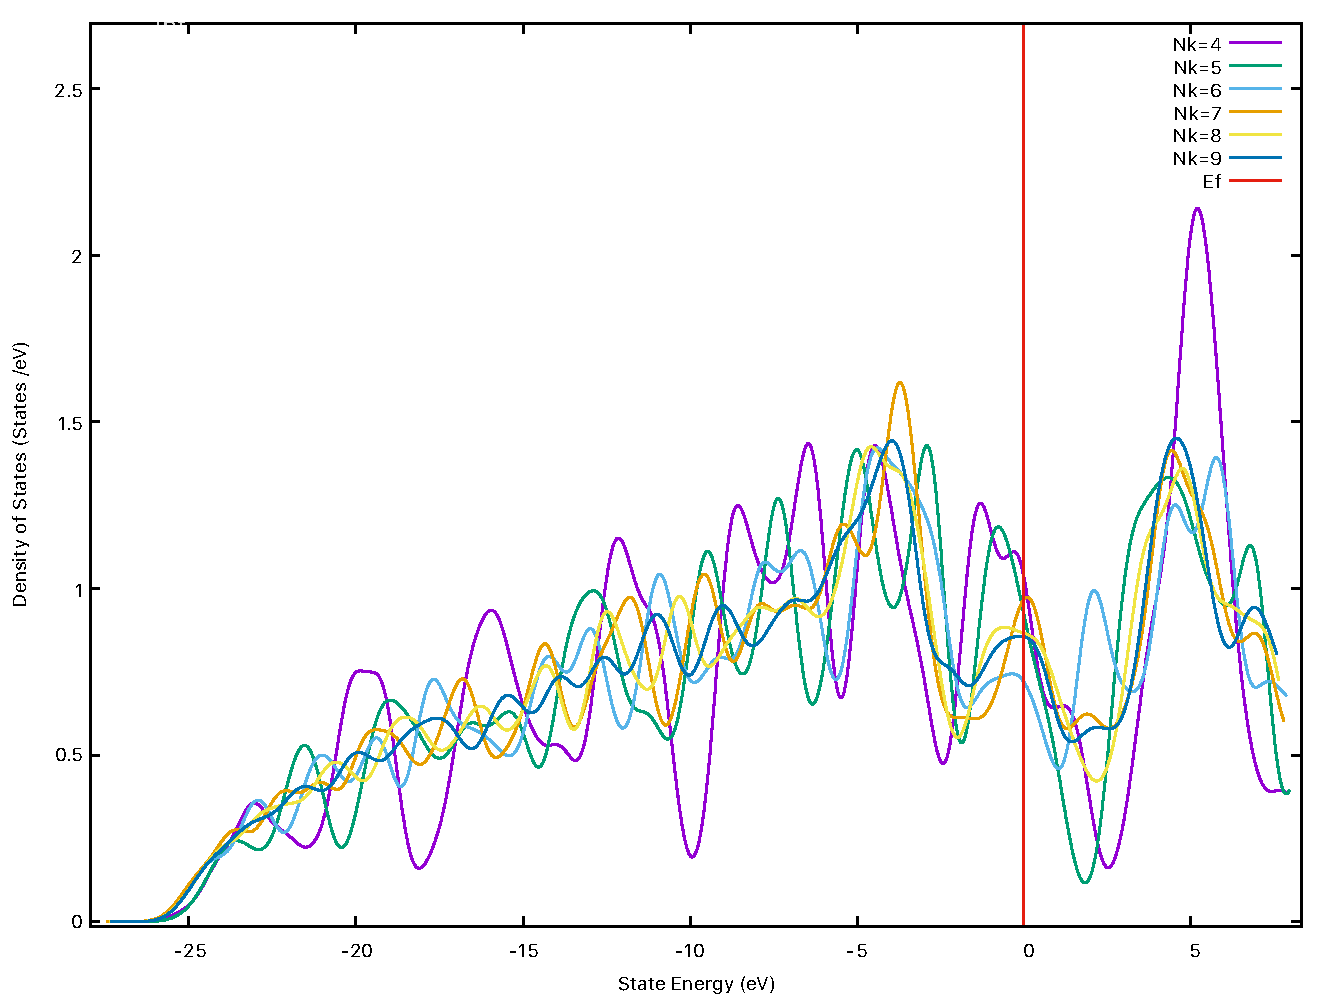
\includegraphics[width=12cm]{dos-conv.pdf}
	\caption{This graph shows various solutions for the density of states when $N_k$ is varied. All results have been shifted so that the Fermi Energy $E_f$ is at 0 eV.}
	\label{fig:dos-conv}
\end{figure}


\begin{figure}[h!!!]
	\centering
	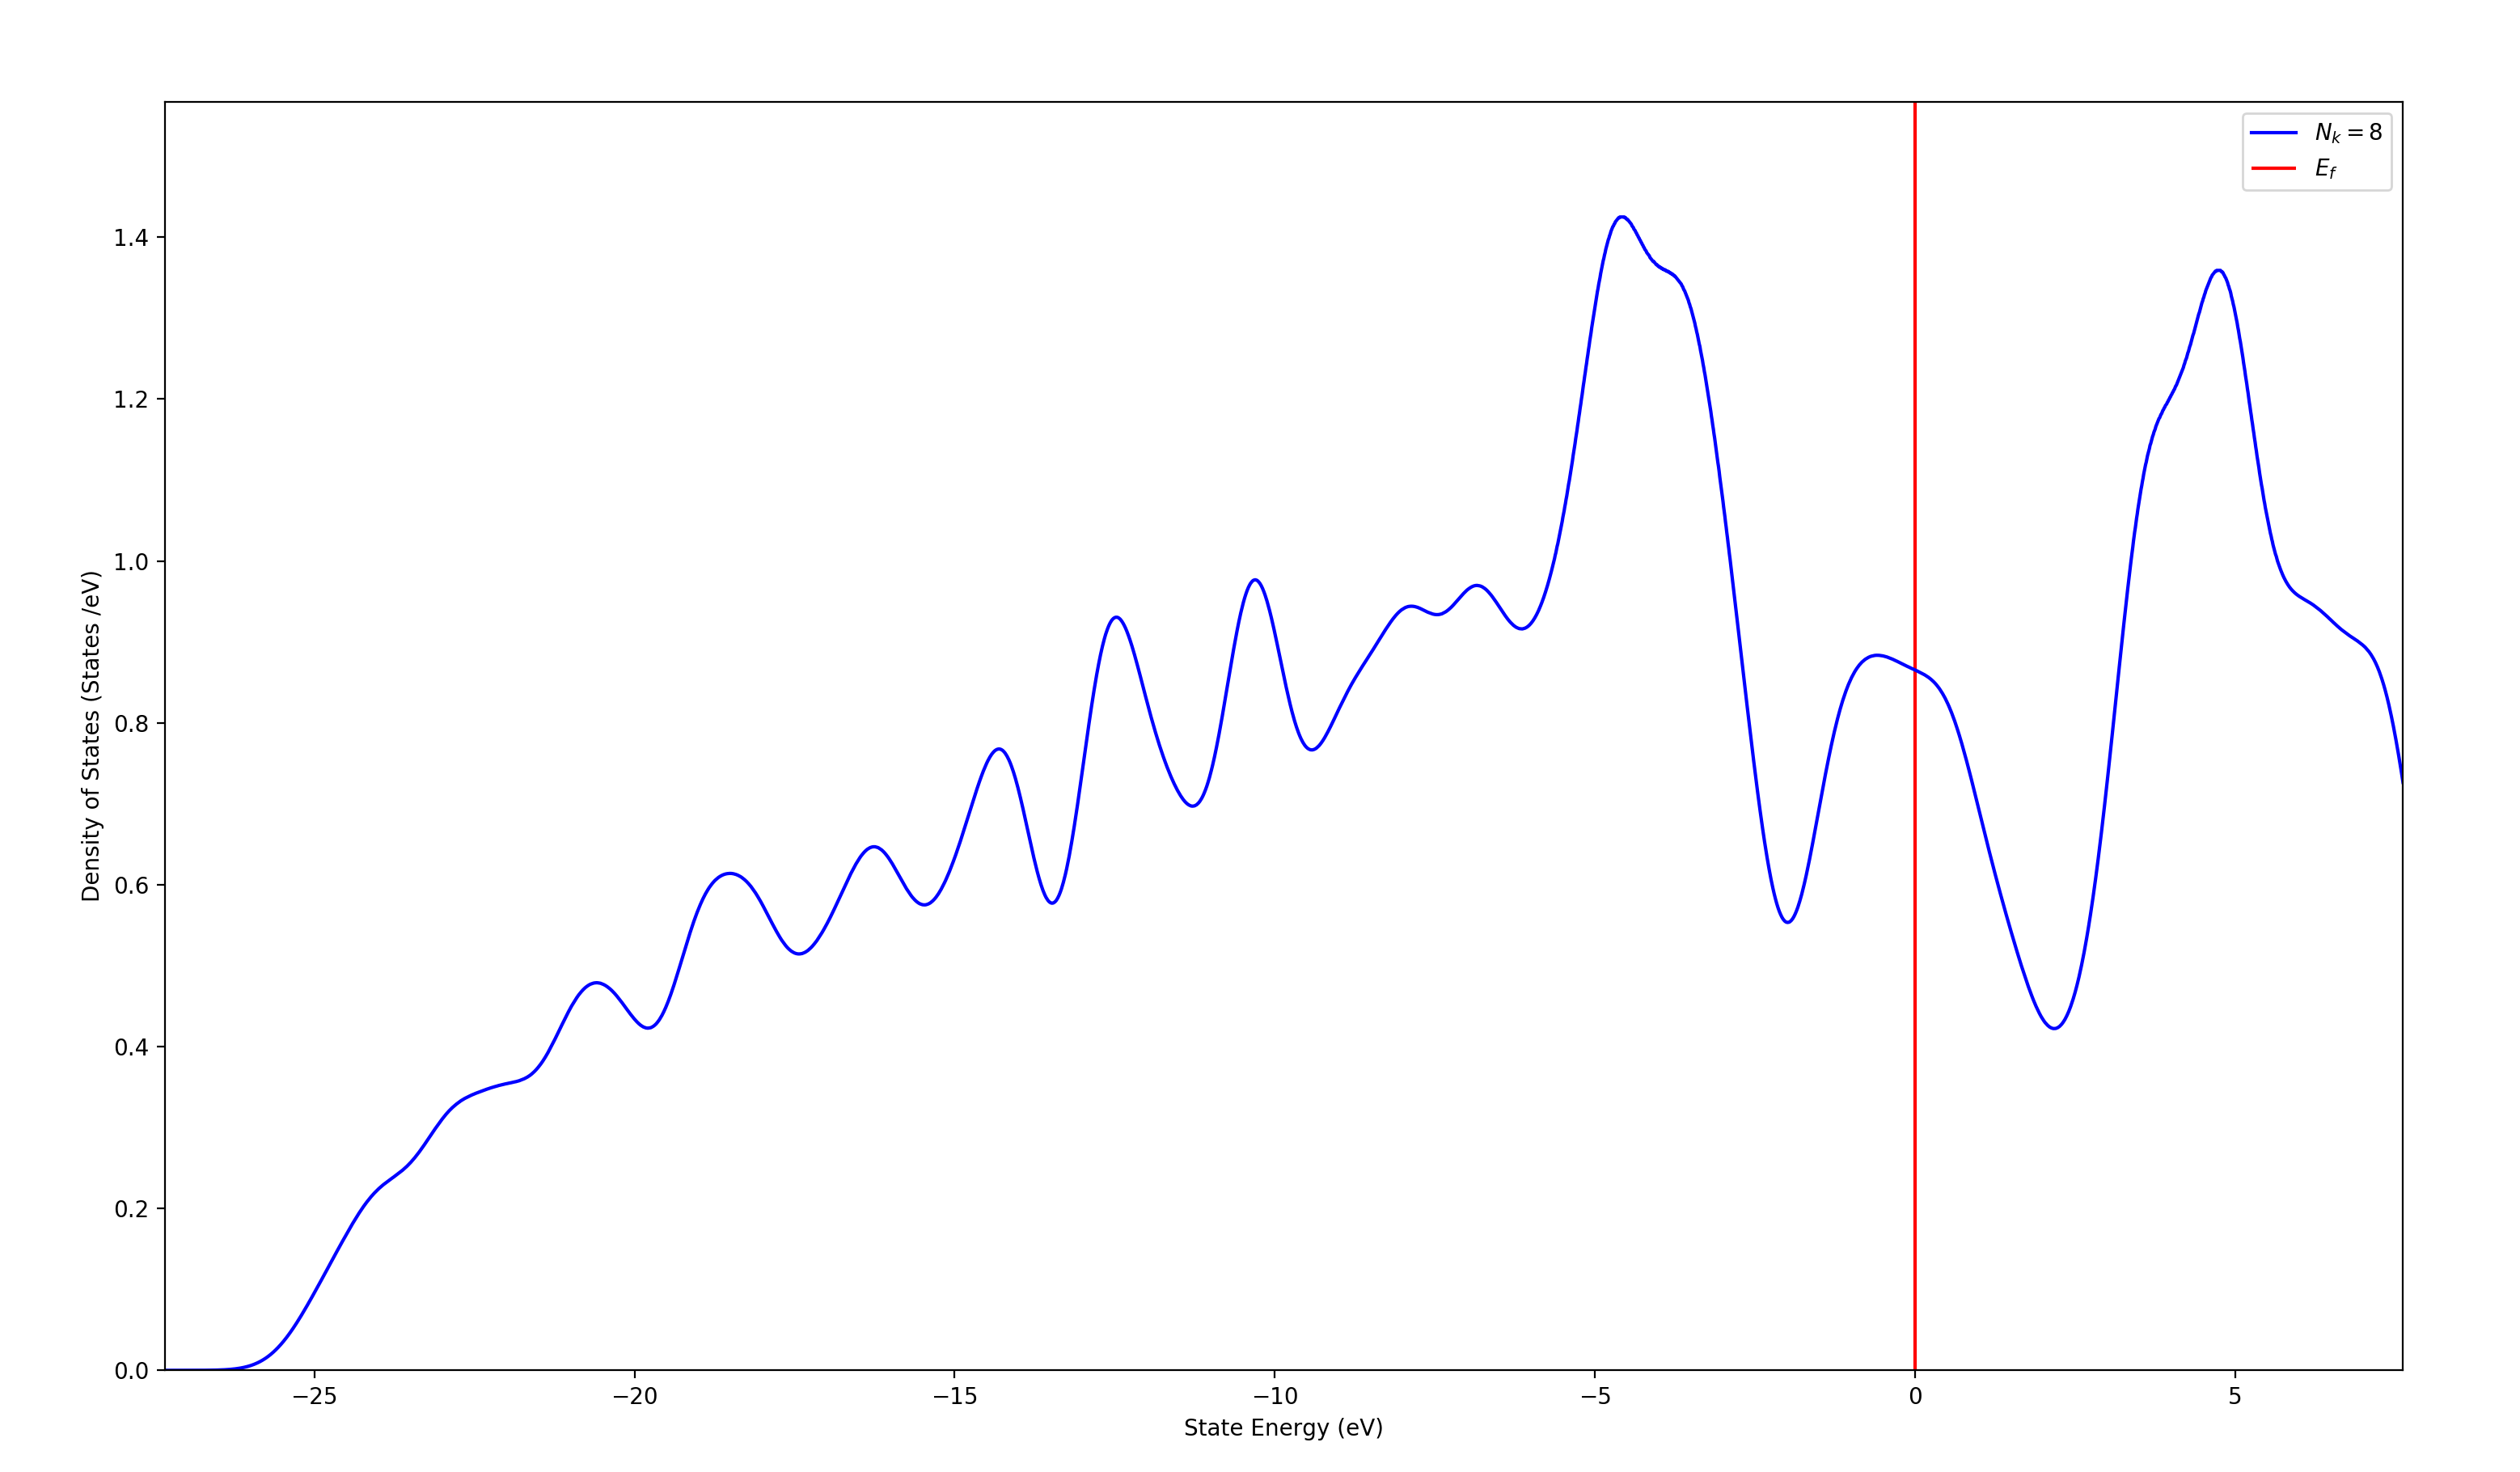
\includegraphics[width=10cm]{dos-final.png}
	\caption{The determined converged solution for the density of states when $N_k=8$. This has also been shifted so that the Fermi Energy $E_f$ is at 0 eV.}
	\label{fig:dos-final}
\end{figure}


\subsection{Stress Tensor Calculation}
The pressure of the system at different $N_k$ values when $E_{cut}=30$ Ry is shown in Table \ref{tab:press}. This was found be carrying out the SCF step at each setting.

\begin{table}[h!!!]
	\centering
	\begin{tabular}{|c|c|}
		\hline
		$N_k$ & Pressure (GPa) \\ \hline
		5     & 201.125        \\ \hline
		8     & 201.248        \\ \hline
	\end{tabular}
	\caption{The results for the pressure of the system when $E_{cut} =30$ Ry and $N_k$ is varied. The pressure is isotropic.}
	\label{tab:press}
\end{table}

\begin{figure}[h!!!!!!!!!!!]
	\centering
	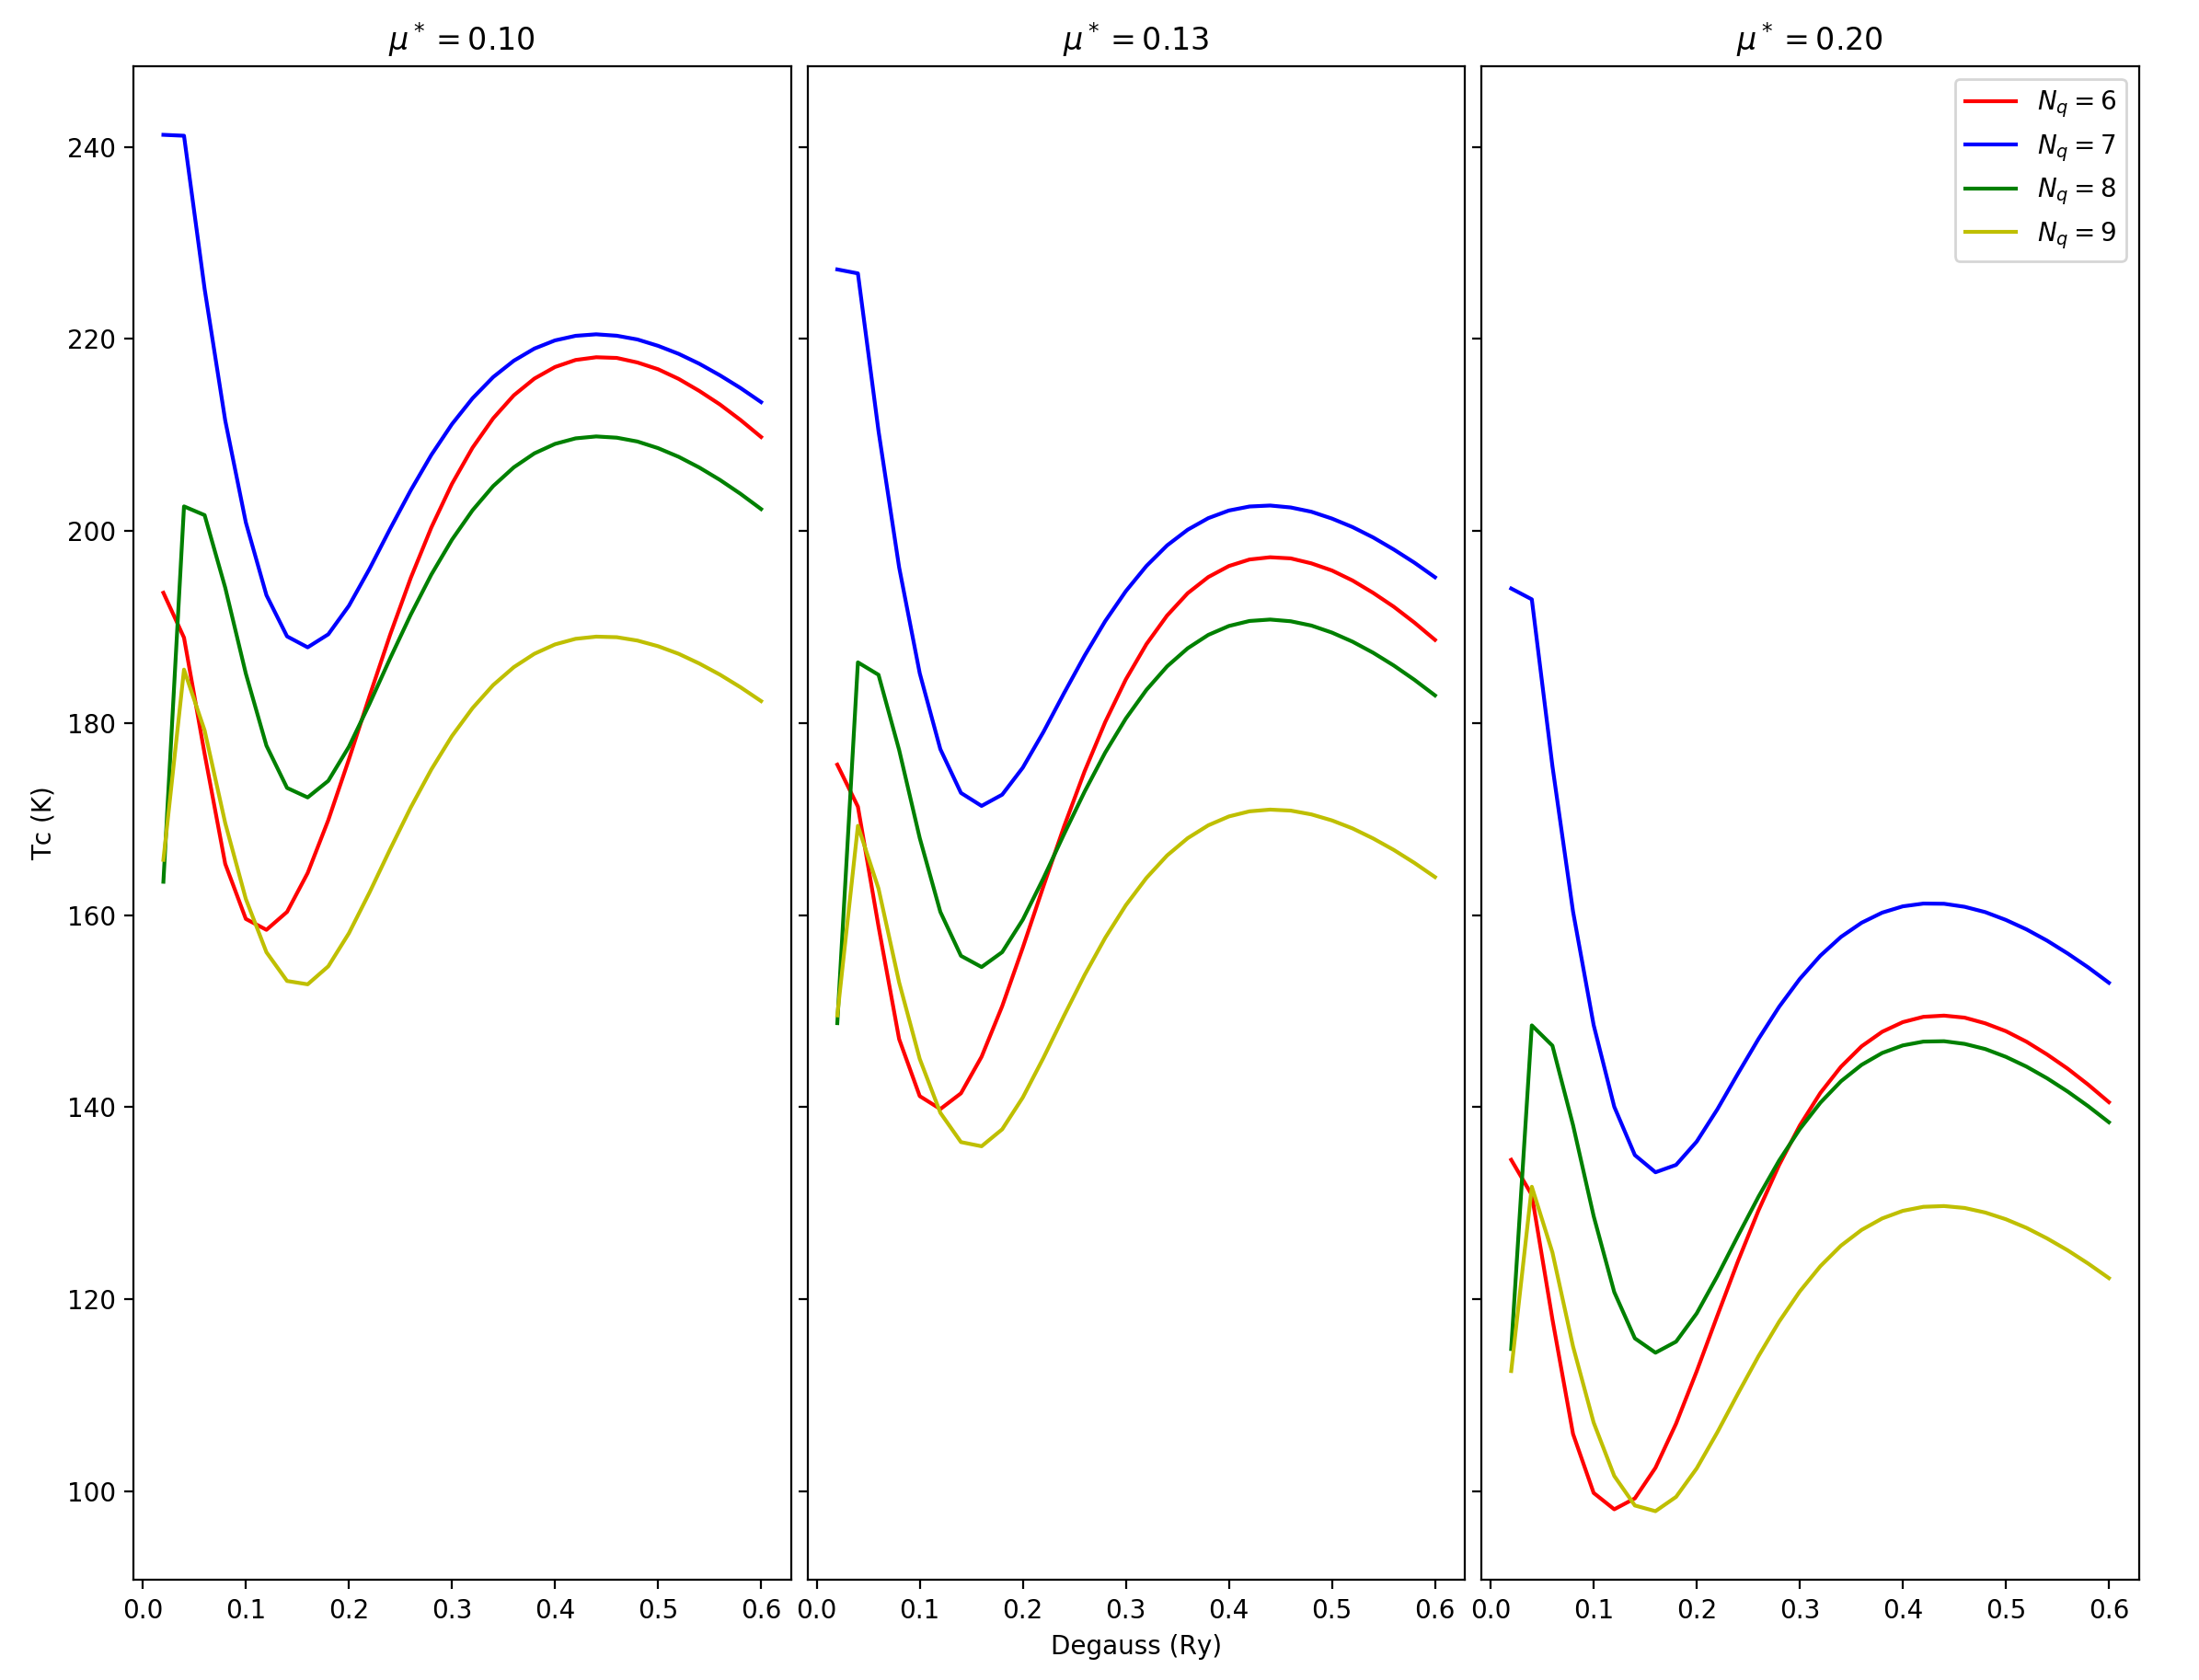
\includegraphics[width=10cm]{Tc_conv-test.png}
	\caption{The results for $T_c$ for various Gaussian smearing values (Degauss) when $N_k$ and $\mu^*$ are also varied.}
	\label{fig:Tc-conv}
\end{figure}

\subsection{DFPT Convergence and $T_c$ Result}
$T_c$ was estimated at various $N_q$ and $\mu^*$ values while $E_{cut}=30$ Ry as shown in Figure \ref{fig:Tc-conv}. Each $N_q$ and $\mu^*$ pair gives a range of estimates for $T_c$ when the Gaussian smearing value, Degauss, is varied. Duan 2014 \cite{duan} found the $T_c = 191$ K to 204 K estimate for $\mu^*=0.10-0.13$ and is the motivation for the choices of $\mu^*$ here. The final value of 0.2 is included for comparison to a higher $\mu^*$ value.


\section{Discussion}
% Structural, electronic properties and superconductivity of H_3S, comparison to literature data
The structure used in this study was the \textit{Im-3m} phase of H$_3$S with lattice parameter $a=2.984 \AA$ at 200 GPa as described in \cite{duan}, shown in \ref{fig:im3m}.

\bigskip

\noindent The results in Figure \ref{fig:E-conv} show the expected decrease in difference from the true value as $E_{cut}$ is increased i.e. more terms in the basis set are used to describe the wavefunction. The 10 meV and 1 meV per atom convergence limits are shown as $E_{cut}= 30$ Ry and 70 Ry respectively, which are reasonable solutions. Throughout the rest of the results $E_{cut}$ is taken to be 30 Ry as 10 meV per atom is the desired convergence here.

\bigskip
\noindent Figure \ref{fig:k-conv} shows a convergence towards the true value as $N_k$ is increased, as expected. It also shows that a convergence of 10 meV per atom is reached when $N_k = 5$, however, $N_k=6$ shows much less convergence with the difference of almost 20 meV per atom from the true solution. This suggests that the convergence when $N_k=5$ is likely a 'lucky' choice of sampling points. This is in agreement with the density of states plot in Figure \ref{fig:dos-conv}. Which shows much variation in the features of the DOS up to $N_k=8$. Particular focus is put on the convergence at $E_f$ as this is important when calculating the Eliashberg function and thus estimating $T_c$. Due to this $N_k=8$ was chosen as the convergence limit over $N_k=7$, as it also shows a good overall convergence throughout the rest of the DOS plot and in the energy convergence in Figure \ref{fig:k-conv}. The determined DOS at $N_K=8$ is then shown independently in Figure \ref{fig:dos-final}. This appears to be in qualitative agreement with the results by Duan \textit{et al} in 2014 \cite{duan}, although this is slightly awkward to compare as they have given the DOS separately for H and S and per formula unit. 

\bigskip
\noindent The stress tensor calculation results in Table \ref{tab:press} show that both $N_k=5$ and $N_k=8$ give an isotropic pressure of 201 GPa, with the $N_k=5$ negligibly closer to the desired 200 GPa. This is in excellent agreement with the expected result with an error of roughly half a percent.

\bigskip
\noindent The results in Figure \ref{fig:Tc-conv} show the estimation of $T_c$ for various $N_q$, $\mu^*$ and Gaussian smearing values. For these solutions $N_k = N_q$ as all points \textbf{\textit{k}}+\textbf{\textit{q}} must also be in the DOS \textbf{\textit{k}}-grid. The data set as a whole shows a higher $T_c$ for lower $\mu^*$ values and a lower $T_c$ for higher $N_q$ values. $N_q=6$ shows a strong dependence on the smearing value as crosses over a range over other $N_q$ results which reflects that it is not a converged solution. This is expected as the $N_k=6$ was found to not be well converged either. The results for $N_q=7$ also depend quite strongly on the smearing value as they show large peaks at small smearing values. $N_q=8$ is the first to show reasonably well converged results, although with slightly extreme minima, which agrees well with the determined $N_k=8$ convergence point determined previously. Ignoring the extreme minima, the results for $N_q=8$ and $\mu^*=0.10$ give a $T_c$ estimate of about 180 K to 210 K, which is in good agreement with the desired results from 2014 of $T_c=$ 191 K to 204 K \cite{duan}. Worth noting is that this paper also found $N_k=8$ to be sufficiently converged, although other parameters had a much higher convergence. 

\bigskip
\noindent Despite finding this agreement, other results do not agree with Duan 2014. Particularly, higher $\mu^*$ values, as seen in the results $\mu^*=0.2$, and higher $N_q$ values. However, Harshman and Fiory in 2017 found the $T_c$ of H$_3$S to be about 180 K \cite{Harshman_2017}, which agrees well with the results for $N_q=9$ and $\mu^*=0.10$ here, which found $T_c=$ 160 K to 180 K. It also agrees well with the $\mu^*=0.13$ and $N_q=8$ results which found $T_c=$ 160 K to 190 K. These results fall short of the 2014 prediction, but only marginally and is likely due to a slight overestimation originally. 

\bigskip
\noindent While the results were marginally overstated, this has evidently prompted much research into hydride type superconductors, such as Lanthanum hydride. As of 2019 the new record $T_c$ is 260 K at 190 GPa \cite{Drozdov_2019, Somayazulu_2019} which is a large improvement on even the predicted $T_c$ of 204 K for H$_3$S. This is also only marginally short of room temperature, with hydrides appearing the key focus to achieve this goal in the future.

\bigskip
\noindent In summary, several convergence checks were carried out on the \textit{Im-3m} phase of H$_3$S with $a=2.984\AA$, finding $E_{cut}=30$ Ry and $N_k=8$ for within 10 meV per atom and achieving a converged DOS. This system was found to have an isotropic pressure of 201 GPa, about half a percent error from the expected 200 GPa. Under BCS theory, with $\mu^*=0.10$ and $N_q=N_k=8$ a $T_c$ estimate was found to be about 180 K to 210 K, which is in good agreement with the key paper, Duan 2014, which found the estimate to be 191 K to 204 K. the 2014 estimate was found with $\mu^*=0.10-0.13$ which is also in agreement with the results found here.

\printbibliography

\end{document}
